\chapter{Systems}
\label{ch:system}
\section{Introduction}
In this section, we will discuss the system setup and the implementation of our complete system(Odometry + SLAM + Place Recognition). First, we discuss the system setup, the sensors used in our system for collecting data. Next, the details of implementation will show how place recognition server integrated to our SLAM system under different modes: online SLAM, offline multimission SLAM map merging, and relocalization. Finally, we further explore the possiblities of open sourcing full pipeline by combining place recognition server with existing open sourced SLAM systems (e.g. FAST-LIO, LIOSAM, etc.) as a future work. 

\section{System Setup}
\label{sec:system_setup}

\subsubsection*{Sensors}
Our system uses Frontier device which comprises a LiDAR, IMU, and three cameras.




\section{Implementations}
\label{sec:implementation}
\subsection*{ROS Framework}

\subsection*{Place Recognition Server}
\subsubsection*{Online SLAM}
Place recognition server is integrated to VILENS odometry and VILENS SLAM node. The place recognition server subscribes to the odometry and LiDAR scan topics from VILENS SLAM node. The place recognition server then publishes service messages to VILENS SLAM node. Service message includes loop candidates and their relative transformation. The online SLAM implementation is shown in \figref{fig:implementation_online_slam}. 
\begin{figure}[t]
  \centering
  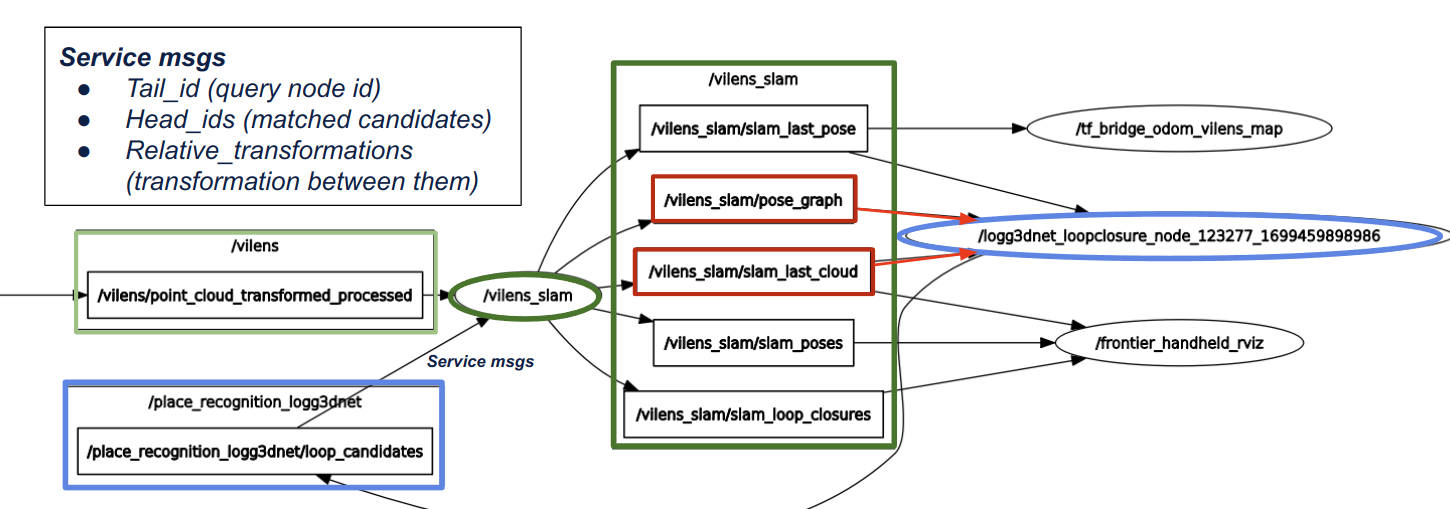
\includegraphics[width=0.99\columnwidth]{pics/Implementation_Online_SLAM.png}
  \caption{Online SLAM Implementation (ROS rqt graph). VILENS odometry and VILENS SLAM( shown in green) are our base system. The place recognition server (shown in blue) subscribe topics from VILENS SLAM node. Then it publishes service messages to VILENS SLAM node. Service message includes loop candidates and their relative transformation.}
  \label{fig:implementation_online_slam}
\end{figure}


\subsubsection*{Offline Multimission SLAM Map Merging}



\subsubsection*{Relocalization}